\chapter{使用样例\label{ch:excample}}
\section{系统起动}
\begin{itemize}
	\item 在桌面找到\textcolor{red}{YQ-500接触热阻综合测试仪.exe}的快捷方式
	\item 在安装路径根目录找到\textcolor{red}{YQ-500接触热阻综合测试仪.exe}应用程序
\end{itemize}
以上两种方式均可打开本软件。
\section{用户登录}
打开本软件后,首先要选择用户模式并登录。本软件有以下两种用户模式:
\begin{itemize}
	\item 普通用户
	\item 高级用户
\end{itemize}
使用者可通过下拉选项选择。
相对\textcolor{red}{普通用户},\textcolor{red}{高级用户}可以进行更多系统级的设置。
在对应栏输入账号密码后,按\textcolor{red}{确认登录}按钮即可进入测试方法选择,
按\textcolor{red}{取消登录}按钮会直接退出本软件(见\figref{fig:exmp_login})。
\begin{figure}[H]
	\centering
	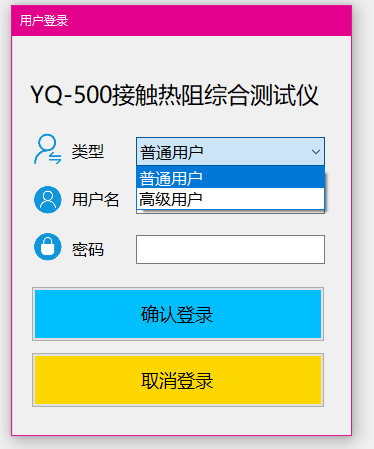
\includegraphics[width=0.6\textwidth]{example/login.png}
	\caption{ 用户登录}
	\label{fig:exmp_login}
\end{figure}
\begin{tips}{账号}{account}
	当前版本不支持用户的注册。在当前版本中\textcolor{red}{普通用户}无需账号密码即可登录,\textcolor{red}{高级用户}的账号密码均为\textcolor{red}{admin}。
\end{tips}

\section{试件热导率测试}
\subsection{测试方法选择}
进入测试方法界面,按\lstinline{导热系数测量}按钮(见\figref{fig:exmp_kappa_chooseMethod})。同时,在每个测试实验里面,
按\lstinline{切换方法}按钮,即可返回到选择测试方法界面(见\figref{fig:exmp_kappa_switchMethod})。
\begin{figure}[htbp]
	\centering
	\includegraphics[width=1\textwidth]{example/KAPPA/chooseMethod.png}
	\caption{ 测试方法选择 \label{fig:exmp_kappa_chooseMethod}}
\end{figure}

\begin{figure}[htbp]
	\centering
	\includegraphics[width=1\textwidth]{example/KAPPA/switchMethod.png}
	\caption{ 切换方法 \label{fig:exmp_kappa_switchMethod}}
\end{figure}

\subsection{参数设置}
用户可根据实验条件,按\lstinline{修改参数}按钮设置参数(见\figref{fig:exmp_kappa_changePara})。
\begin{figure}[htbp]
	\centering
	\includegraphics[width=1\textwidth]{example/KAPPA/changePara.png}
	\caption{ 修改参数 \label{fig:exmp_kappa_changePara}}
\end{figure}
在修改参数时,\lstinline{高级用户}可以设置全部实验条件信息,而\lstinline{普通用户}只可以设置试件的测温探头位置、通道编号、
样品截面积和加载压力等信息,设置完成按\lstinline{确认参数}按钮保存(见\figref{fig:exmp_kappa_changeParaEnable})。
\begin{note}
没有使用的测温探头,其位置和通道编号需要填入\lstinline{*}作为参数。
同时,测温探头的位置参数应按照\lstinline{现场测试的两相邻测温探头距离}要求严格填写。
\end{note}
\begin{figure}[htbp]
	\centering
	\includegraphics[width=0.9\textwidth]{example/KAPPA/changeParaEnable.png}
	\caption{ 确定参数修改 \label{fig:exmp_kappa_changeParaEnable}}
\end{figure}
~\\
\subsection{执行测试}
用户设计完参数后,按\lstinline{运行}按钮即可开始实验测试(见\figref{fig:exmp_kappa_run})。
\begin{figure}[htbp]
	\centering
	\includegraphics[width=1\textwidth]{example/KAPPA/run.png}
	\caption{ 运行 \label{fig:exmp_kappa_run}}
\end{figure}
在运行的时候,按\lstinline{温度监控}按钮即可显示实时的探头温度信息见(\figref{fig:exmp_kappa_tempMirror})。
\begin{figure}[htbp]
	\centering
	\includegraphics[width=1\textwidth]{example/KAPPA/tempMirror.png}
	\caption{ 温度监视图表 \label{fig:exmp_kappa_tempMirror}}
\end{figure}
\lstinline{温度监控}可实时显示各测温探头温度,上部为各通道图例,可对其进行显示或隐藏,
左下角可设置\lstinline{实时/全局显示}和\lstinline{纵轴放大},右上角按\lstinline{隐藏图表}按钮可对其隐藏。
特别的,勾选\lstinline{纵轴放大},再用鼠标按压左键框选,可实现纵轴放大,若想恢复原始范围,
点击左上角滚轴\lstinline{'-'}即可;鼠标指向温度线时,可捕获其通道编号、采集时间和温度信息(见\figref{fig:exmp_kappa_chartEdit})。\\
\begin{figure}[htbp]
	\centering
	\includegraphics[width=0.9\textwidth]{example/KAPPA/chartEdit.png}
	\caption{ 图表显示设置 \label{fig:exmp_kappa_chartEdit}}
\end{figure}

\subsection{获取测试结果}
	当温度曲线稳定,按\lstinline{当前测试}按钮即可自动求得结果(见\figref{fig:exmp_kappa_currentTest})。
\begin{note}
	软件通过数采仪获取一定数量的数据才可以计算,同时为了保证实验的准确性,应等待温度相对稳定在某一范围
再点击\lstinline{当前测试}按钮计算结果。
\end{note}
\begin{figure}[htbp]
	\centering
	\includegraphics[width=0.9\textwidth]{example/KAPPA/currentTest.png}
	\caption{ 当前测试结果 \label{fig:exmp_kappa_currentTest}}
\end{figure}
软件可处理历史采集的实验数据,默认历史数据保存在安装根目录下\lstinline{AutoSave}的文件中,
选择\lstinline{(.rst)类型}文件,即可自动计算实验结果(见\figref{fig:exmp_historicalTest})。得到实验结果后,
按\lstinline{导出结果}按钮,将实验结果以图片形式保存(见\figref{fig:exmp_exportResult})。
\begin{figure}[htbp]
	\centering
	\includegraphics[width=0.9\textwidth]{example/KAPPA/historicalTest.png}
	\caption{ 历史测试结果 \label{fig:exmp_kappa_historicalTest}}
\end{figure}

\begin{figure}[htbp]
	\centering
	\includegraphics[width=0.9\textwidth]{example/KAPPA/exportResult.png}
	\caption{ 导出测试结果 \label{fig:exmp_kappa_exportResult}}
\end{figure}
\section{固-固试件间接触热阻测试}
\subsection{测试方法选择}
进入测试方法界面,按\textcolor{red}{导热系数测量}按钮(见\figref{fig:exmp_itc_chooseMethod})。同时,在每个测试实验里面,
按\textcolor{red}{切换方法}按钮,即可返回到选择测试方法界面(见\figref{fig:exmp_itc_switchMethod})。
\begin{figure}[H]
	\centering
	\includegraphics[width=1\textwidth]{example/ITC/chooseMethod.png}
	\caption{ 测试方法选择 \label{fig:exmp_itc_chooseMethod}}
\end{figure}

\begin{figure}[H]
	\centering
	\includegraphics[width=1\textwidth]{example/ITC/switchMethod.png}
	\caption{ 切换方法 \label{fig:exmp_itc_switchMethod}}
\end{figure}

\subsection{参数设置}
用户可根据实验条件,按\textcolor{red}{修改参数}按钮设置参数(见\figref{fig:exmp_itc_changePara})。
\begin{figure}[H]
	\centering
	\includegraphics[width=1\textwidth]{example/ITC/changePara.png}
	\caption{ 修改参数 \label{fig:exmp_itc_changePara}}
\end{figure}
在修改参数时,\textcolor{red}{高级用户}可以设置全部实验条件信息,而\textcolor{red}{普通用户}只可以设置试件的测温探头位置、通道编号、
样品截面积和加载压力等信息,设置完成按\textcolor{red}{确认参数}按钮保存(见\figref{fig:exmp_itc_changeParaEnable})。
\begin{tips}{未启用的探头}
没有使用的测温探头,其位置和通道编号需要填入\textcolor{red}{*}作为参数。
同时,测温探头的位置参数应按照\textcolor{red}{现场测试的两相邻测温探头距离}要求严格填写。
\end{tips}
\begin{figure}[H]
	\centering
	\includegraphics[width=0.9\textwidth]{example/ITC/changeParaEnable.png}
	\caption{ 确定参数修改 \label{fig:exmp_itc_changeParaEnable}}
\end{figure}

\subsection{执行测试}
用户设计完参数后,按\textcolor{red}{运行}按钮即可开始实验测试(见\figref{fig:exmp_itc_run})。
\begin{figure}[H]
	\centering
	\includegraphics[width=1\textwidth]{example/ITC/run.png}
	\caption{ 运行 \label{fig:exmp_itc_run}}
\end{figure}
在运行的时候,按\textcolor{red}{温度监控}按钮即可显示实时的探头温度信息见(\figref{fig:exmp_itc_tempMirror})。
\begin{figure}[H]
	\centering
	\includegraphics[width=1\textwidth]{example/ITC/tempMirror.png}
	\caption{ 温度监视图表 \label{fig:exmp_itc_tempMirror}}
\end{figure}
\textcolor{red}{温度监控}可实时显示各测温探头温度,上部为各通道图例,可对其进行显示或隐藏,
左下角可设置\textcolor{red}{实时/全局显示}和\textcolor{red}{纵轴放大},右上角按\textcolor{red}{隐藏图表}按钮可对其隐藏。
特别的,勾选\textcolor{red}{纵轴放大},再用鼠标按压左键框选,可实现纵轴放大,若想恢复原始范围,
点击左上角滚轴\textcolor{red}{'-'}即可;鼠标指向温度线时,可捕获其通道编号、采集时间和温度信息(见\figref{fig:exmp_itc_chartEdit})。\\
\begin{figure}[H]
	\centering
	\includegraphics[width=0.9\textwidth]{example/ITC/chartEdit.png}
	\caption{ 图表显示设置 \label{fig:exmp_itc_chartEdit}}
\end{figure}

\subsection{获取测试结果}
	当温度曲线稳定,按\textcolor{red}{当前测试}按钮即可自动求得结果(见\figref{fig:exmp_itc_currentTest})。
\begin{tips}{结果计算}
	软件通过数采仪获取一定数量的数据才可以计算,同时为了保证实验的准确性,应等待温度相对稳定在某一范围
再点击\textcolor{red}{当前测试}按钮计算结果。
\end{tips}
\begin{figure}[H]
	\centering
	\includegraphics[width=0.9\textwidth]{example/ITC/currentTest.png}
	\caption{ 当前测试结果 \label{fig:exmp_itc_currentTest}}
\end{figure}
软件可处理历史采集的实验数据,默认历史数据保存在安装根目录下\textcolor{red}{AutoSave}的文件中,
选择\textcolor{red}{(.rst)类型}文件,即可自动计算实验结果(见\figref{fig:exmp_itc_historicalTest})。得到实验结果后,
按\textcolor{red}{导出结果}按钮,将实验结果以图片形式保存(见\figref{fig:exmp_itc_exportResult})。
\begin{figure}[H]
	\centering
	\includegraphics[width=0.9\textwidth]{example/ITC/historicalTest.png}
	\caption{ 历史测试结果 \label{fig:exmp_itc_historicalTest}}
\end{figure}

\begin{figure}[H]
	\centering
	\includegraphics[width=0.9\textwidth]{example/ITC/exportResult.png}
	\caption{ 导出测试结果 \label{fig:exmp_itc_exportResult}}
\end{figure}
\section{热流计间热界面材料测试}
\section{固-固试件间热界面材料测试}
\subsection{测试方法选择}
进入测试方法界面,按\textcolor{red}{导热系数测量}按钮(见\figref{fig:exmp_itms_chooseMethod})。同时,在每个测试实验里面,
按\textcolor{red}{切换方法}按钮,即可返回到选择测试方法界面(见\figref{fig:exmp_itms_switchMethod})。
\begin{figure}[htbp]
	\centering
	\includegraphics[width=1\textwidth]{example/ITMS/chooseMethod.png}
	\caption{ 测试方法选择 \label{fig:exmp_itms_chooseMethod}}
\end{figure}

\begin{figure}[htbp]
	\centering
	\includegraphics[width=1\textwidth]{example/ITMS/switchMethod.png}
	\caption{ 切换方法 \label{fig:exmp_itms_switchMethod}}
\end{figure}

\subsection{参数设置}
用户可根据实验条件,按\textcolor{red}{修改参数}按钮设置参数(见\figref{fig:exmp_itms_changePara})。
\begin{figure}[htbp]
	\centering
	\includegraphics[width=1\textwidth]{example/ITMS/changePara.png}
	\caption{ 修改参数 \label{fig:exmp_itms_changePara}}
\end{figure}
在修改参数时,\textcolor{red}{高级用户}可以设置全部实验条件信息,而\textcolor{red}{普通用户}只可以设置试件的测温探头位置、通道编号、
样品截面积和加载压力等信息,设置完成按\textcolor{red}{确认参数}按钮保存(见\figref{fig:exmp_itms_changeParaEnable})。
\begin{note}
没有使用的测温探头,其位置和通道编号需要填入\textcolor{red}{*}作为参数。
同时,测温探头的位置参数应按照\textcolor{red}{现场测试的两相邻测温探头距离}要求严格填写。
\end{note}
\begin{figure}[htbp]
	\centering
	\includegraphics[width=0.9\textwidth]{example/ITMS/changeParaEnable.png}
	\caption{ 确定参数修改 \label{fig:exmp_itms_changeParaEnable}}
\end{figure}
~\\
\subsection{执行测试}
用户设计完参数后,按\textcolor{red}{运行}按钮即可开始实验测试(见\figref{fig:exmp_itms_run})。
\begin{figure}[htbp]
	\centering
	\includegraphics[width=1\textwidth]{example/ITMS/run.png}
	\caption{ 运行 \label{fig:exmp_itms_run}}
\end{figure}
在运行的时候,按\textcolor{red}{温度监控}按钮即可显示实时的探头温度信息见(\figref{fig:exmp_itms_tempMirror})。
\begin{figure}[htbp]
	\centering
	\includegraphics[width=1\textwidth]{example/ITMS/tempMirror.png}
	\caption{ 温度监视图表 \label{fig:exmp_itms_tempMirror}}
\end{figure}
\textcolor{red}{温度监控}可实时显示各测温探头温度,上部为各通道图例,可对其进行显示或隐藏,
左下角可设置\textcolor{red}{实时/全局显示}和\textcolor{red}{纵轴放大},右上角按\textcolor{red}{隐藏图表}按钮可对其隐藏。
特别的,勾选\textcolor{red}{纵轴放大},再用鼠标按压左键框选,可实现纵轴放大,若想恢复原始范围,
点击左上角滚轴\textcolor{red}{'-'}即可;鼠标指向温度线时,可捕获其通道编号、采集时间和温度信息(见\figref{fig:exmp_itms_chartEdit})。\\
\begin{figure}[htbp]
	\centering
	\includegraphics[width=0.9\textwidth]{example/ITMS/chartEdit.png}
	\caption{ 图表显示设置 \label{fig:exmp_itms_chartEdit}}
\end{figure}

\subsection{获取测试结果}
	当温度曲线稳定,按\textcolor{red}{当前测试}按钮即可自动求得结果(见\figref{fig:exmp_itms_currentTest})。
\begin{note}
	软件通过数采仪获取一定数量的数据才可以计算,同时为了保证实验的准确性,应等待温度相对稳定在某一范围
再点击\textcolor{red}{当前测试}按钮计算结果。
\end{note}
\begin{figure}[htbp]
	\centering
	\includegraphics[width=0.9\textwidth]{example/ITMS/currentTest.png}
	\caption{ 当前测试结果 \label{fig:exmp_itms_currentTest}}
\end{figure}
软件可处理历史采集的实验数据,默认历史数据保存在安装根目录下\textcolor{red}{AutoSave}的文件中,
选择\textcolor{red}{(.rst)类型}文件,即可自动计算实验结果(见\figref{fig:exmp_itms_historicalTest})。得到实验结果后,
按\textcolor{red}{导出结果}按钮,将实验结果以图片形式保存(见\figref{fig:exmp_itms_exportResult})。
\begin{figure}[htbp]
	\centering
	\includegraphics[width=0.9\textwidth]{example/ITMS/historicalTest.png}
	\caption{ 历史测试结果 \label{fig:exmp_itms_historicalTest}}
\end{figure}

\begin{figure}[htbp]
	\centering
	\includegraphics[width=0.9\textwidth]{example/ITMS/exportResult.png}
	\caption{ 导出测试结果 \label{fig:exmp_itms_exportResult}}
\end{figure}

% \section{高级设置}
% \begin{tips}
% 	出厂已设置好,不要随意更改。
% \end{tips}
% \subsection{高级用户模式登录}
% 打开本软件后,首先要选择\textcolor{red}{高级用户}模式并登录。\textcolor{red}{高级用户}的账号密码均为\textcolor{red}{admin},
% 详见\ref{subsec:Advance}一节。
% \subsection{测试方法选择}
% 高级模式下的参数修改,可以选择任意一种测试方法进入(见\figref{fig:advance_chooseMethod})。
% \begin{figure}[H]
% 	\centering
% 	\includegraphics[width=1\textwidth]{example/Advance/chooseMethod.png}
% 	\caption{ 测试方法选择\label{fig:advance_chooseMethod}}
% \end{figure}

% \subsection{参数设置}
% \textcolor{red}{高级用户}可以设置全部实验条件信息,包括设置热流量计和试件的测温探头位置、通道编号、
% 样品截面积和加载压力等信息,设置完成按\textcolor{red}{确认参数}按钮保存(见\figref{fig:advance_changePara})。
% \begin{figure}[H]
% 	\centering
% 	\includegraphics[width=1\textwidth]{example/Advance/changePara.png}
% 	\caption{ 修改参数 \label{fig:advance_changePara}}
% \end{figure}

% \subsection{串口设置}
% \textcolor{red}{高级用户}可以设置串口编号、波特率和保存数据间隔等,
% 设置完成按\textcolor{red}{确认}按钮保存(见\figref{fig:advance_serialPort})。
% \begin{figure}[H]
% 	\centering
% 	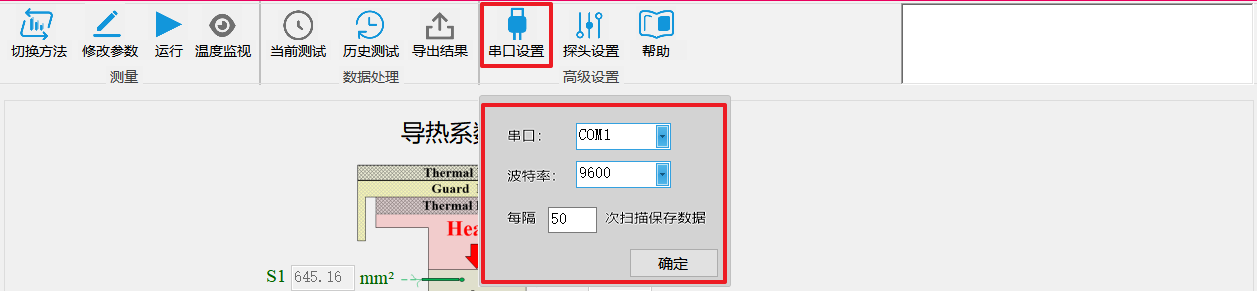
\includegraphics[width=1\textwidth]{example/Advance/serialPort.png}
% 	\caption{ 设置串口 \label{fig:advance_serialPort}}
% \end{figure}

% \subsection{标定参数设置}
% \textcolor{red}{高级用户}可以设置测温探头类型、标定参数等信息。不用的类型的
% 测温探头,有对应的拟合标定方程。输入对应的标定按\textcolor{red}{确认修改}按
% 钮保存(见\figref{fig:advance_settingPara})。
% \begin{figure}[H]
% 	\centering
% 	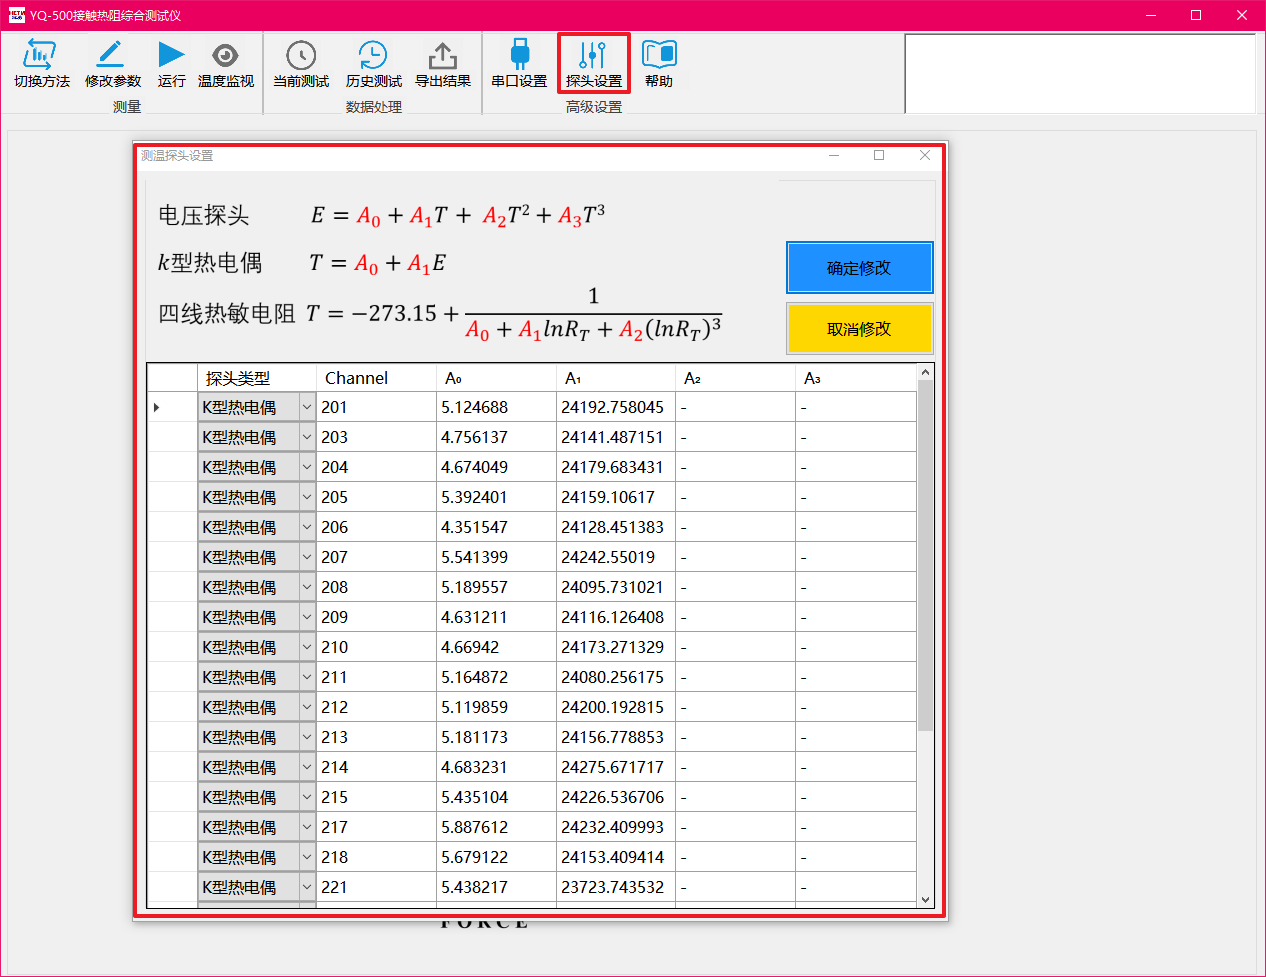
\includegraphics[width=1\textwidth]{example/Advance/settingPara.png}
% 	\caption{ 标定设置 \label{fig:advance_settingPara}}
% \end{figure}
% 设置成功之后,之前的旧版本标定参数会备份在相关路径(见\figref{fig:advance_backupPara})。
% \begin{figure}[H]
% 	\centering
% 	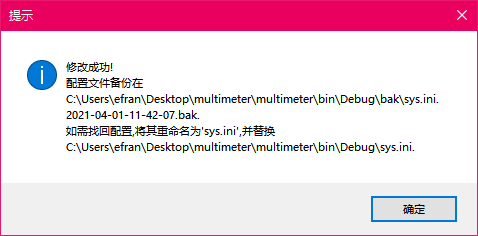
\includegraphics[width=1\textwidth]{example/Advance/backupPara.png}
% 	\caption{ 备份路径 \label{fig:advance_backupPara}}
% \end{figure}






